\section{Использование управления в скользящих режимах}\label{sec:ch3/sec3}

\subsection*{Теоретические основы управления в скользящих режимах}\label{subsec:ch3/sec3/sub1}

Управление в скользящих режимах представляет собой метод управления нелинейными системами, который особенно
эффективен в условиях неопределенностей и нелинейностей, характерных для пневматических систем.
Концепция данного метода основана на принудительном переводе рабочей точки динамической
системы на заранее заданную поверхность в пространстве состояний
и последующем удержании её в окрестности этой поверхности.

Представим физический смысл данного подхода на примере позиционного пневмопривода.
Допустим, мы хотим переместить шток пневмоцилиндра из текущего положения $x$ в заданное $x_d$.
Состояние системы в любой момент времени можно охарактеризовать двумя параметрами:
ошибкой позиционирования $e = x_d - x$ и скоростью изменения этой ошибки $\dot{e} = -\dot{x}$
(т.е. скоростью движения штока с обратным знаком). На фазовой плоскости $(e, \dot{e})$ текущее состояние системы изображается
точкой, а её движение – траекторией, согласно рисунку~\ref{fig:phase_plane}.

\begin{figure}[ht]
	\centerfloat{
		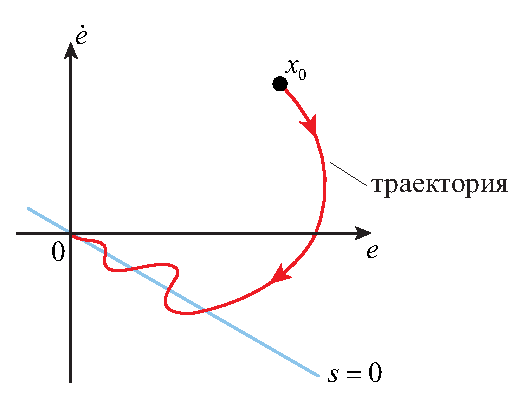
\includegraphics[]{part3/phase_plane.eps}
	}
	\caption{Иллюстрация принципа управления в скользящих режимах: $s=0$ -- поверхность скольжения; $S^+$ и $S^-$ -- области притяжения к поверхности скольжения}
	\label{fig:phase_plane}
\end{figure}

Ключевая идея управления в скользящих режимах заключается в
определении на фазовой плоскости линии (или в общем случае многомерной поверхности), называемой \textit{поверхностью скольжения}, которая описывается уравнением:
\begin{equation}
	s(e, \dot{e}) = 0,
\end{equation}
где $s(e, \dot{e})$ -- некоторая функция, связывающая ошибку позиционирования и скорость.
\nomenclature{$s(e, \dot{e})$}{Функция поверхности скольжения\nomrefeqpage}

Наиболее простой случай -- линейная функция:
\begin{equation}
	s = \dot{e} + \lambda e,
\end{equation}
где $\lambda > 0$ -- параметр, определяющий скорость сходимости ошибки к нулю.
\nomenclature{$\lambda$}{Параметр скорости сходимости ошибки к нулю\nomrefeqpage}

После определения функции $s$ вся фазовая плоскость делится на
две области: $s > 0$ и $s < 0$. Для каждой из этих областей выбирается своё управляющее
воздействие, которое принудительно направляет траекторию системы к поверхности скольжения. Когда траектория достигает
поверхности, система начинает двигаться вдоль неё к состоянию с нулевой ошибкой $(e, \dot{e}) = (0, 0)$.

В случае пневмопривода с дискретными распределителями можно использовать следующий закон управления:
\begin{equation}
	\mathbf{u} = \begin{cases}
		[1,0,0,1], & s > \varepsilon;      \\
		[0,0,0,0], & |s| \leq \varepsilon; \\
		[0,1,1,0], & s < -\varepsilon,
	\end{cases}
\end{equation}
где $\varepsilon > 0$ -- малый параметр, определяющий ширину «коридора» вокруг поверхности скольжения; $[1,0,0,1]$ -- комбинация состояний
распределителей, обеспечивающая максимальное ускорение в положительном направлении; $[0,1,1,0]$ -- комбинация, обеспечивающая максимальное
ускорение в отрицательном направлении; $[0,0,0,0]$ -- все распределители закрыты.
\nomenclature{$\varepsilon$}{Малый параметр, определяющий ширину <<коридора>> вокруг поверхности скольжения\nomrefeqpage}

При движении к поверхности скольжения выбирается режим максимального ускорения (положительного или отрицательного, в зависимости
от знака $s$). Когда система попадает в $\varepsilon$-окрестность поверхности ($|s| \leq \varepsilon$), все распределители закрываются,
что приводит к торможению штока под действием сил трения и пневматической жёсткости (сжатый воздух в закрытых полостях действует как пружина).

Этот принцип управления обеспечивает робастность (устойчивость к возмущениям) и простоту реализации, что делает его особенно
привлекательным для систем с дискретными исполнительными элементами, такими как пневмоприводы с дискретными распределителями.

\subsection*{Многорежимное управление в скользящих режимах}\label{subsec:ch3/sec3/sub2}

При практической реализации управления в скользящих режимах для пневмопривода с дискретными распределителями возникает
ряд проблем, связанных с динамикой системы. Базовая трёхрежимная схема, хотя и обеспечивает достижение целевого положения,
но может приводить к возникновению колебаний вблизи заданной позиции, что снижает точность позиционирования и увеличивает износ распределителей.

Для преодоления этих недостатков предлагается использовать многорежимное управление (5 и 7 режимов), обеспечивающее
более плавное торможение при подходе к целевому положению. В данном разделе рассматриваются особенности
таких схем управления и их преимущества по сравнению с базовой трёхрежимной схемой.

\textbf{Трёхрежимное управление.}
Базовая схема управления в скользящих режимах для пневмопривода с дискретными распределителями предусматривает три режима работы:
\begin{enumerate}
	\item \textbf{Режим максимального положительного ускорения} $[1,0,0,1]$: поршневая полость соединена с источником питания, штоковая -- с атмосферой. Этот режим обеспечивает максимальное ускорение штока в положительном направлении.
	\item \textbf{Режим максимального отрицательного ускорения} $[0,1,1,0]$: поршневая полость соединена с атмосферой, штоковая -- с источником питания. Этот режим обеспечивает максимальное ускорение штока в отрицательном направлении.
	\item \textbf{Режим удержания} $[0,0,0,0]$: обе полости изолированы от источника питания и атмосферы. Этот режим обеспечивает торможение и удержание штока за счёт пневматической жёсткости и сил трения.
\end{enumerate}

Закон переключения между режимами определяется значением функции переключения $s = \dot{e} + \lambda e$:
\begin{equation}
	\mathbf{u}(s) = \begin{cases}
		[1,0,0,1], & s > \varepsilon;      \\
		[0,0,0,0], & |s| \leq \varepsilon; \\
		[0,1,1,0], & s < -\varepsilon,
	\end{cases}
\end{equation}
где $\varepsilon > 0$ -- параметр, определяющий ширину зоны переключения.
\nomenclature{$\varepsilon$}{Ширина зоны переключения\nomrefeqpage}

В фазовом пространстве векторное поле системы разделяется на три области линией переключения $s = 0$, представленные на рисунке~\ref{fig:vector_field_linear}.
В области $s > \varepsilon$ векторы скоростей направлены к линии переключения под действием управления $\mathbf{u} = [1,0,0,1]$.
При $s < -\varepsilon$ управление $\mathbf{u} = [0,1,1,0]$ формирует векторное поле, обеспечивающее движение к линии
переключения с противоположной стороны. В зоне $|s| \leq \varepsilon$ все распределители закрыты $\mathbf{u} = [0,0,0,0]$, что приводит к замедлению движения.

\begin{figure}[ht]
	\centering
	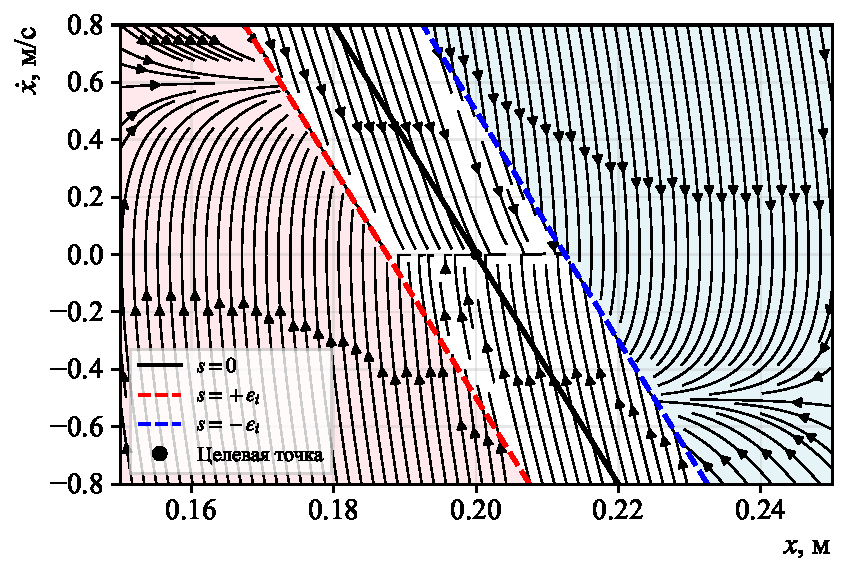
\includegraphics[]{part3/phase_portrait_3mode.pdf}
	\caption{Распределение векторного поля в фазовом пространстве для трёхрежимного управления. Стрелками показаны направления
		движения в различных областях фазовой плоскости, пунктирными линиями -- границы переключения режимов}
	\label{fig:vector_field_linear}
\end{figure}

При малых значениях параметра $\varepsilon$ в системе может возникать эффект <<дребезга>> (chattering),
обусловленный конечным быстродействием электромагнитных распределителей и инерционностью процессов.
На рисунке~\ref{fig:ch3:transient_comparison_linear_mode3} представлены результаты моделирования
для двух значений параметра $\varepsilon$.

\begin{figure}[ht]
	\centering
	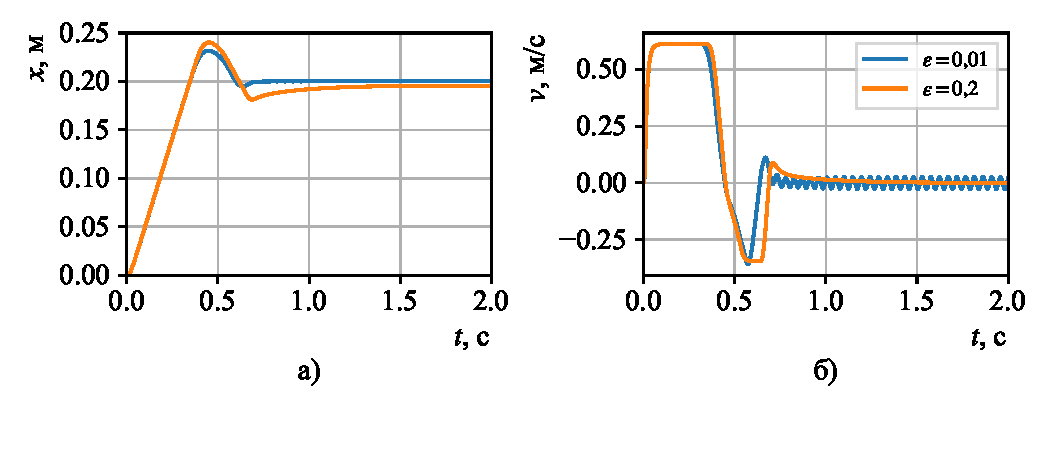
\includegraphics[]{part3/sliding_mode_linear_transients.pdf}
	\caption{Переходные процессы для трёхрежимного управления с различными значениями параметра $\varepsilon$.
		При малом значении $\varepsilon = \num{0.01}$ (синяя линия) наблюдаются колебания,
		при большем значении $\varepsilon = \num{0.2}$ (красная линия) процесс становится апериодическим, но с большей статической ошибкой}
	\label{fig:ch3:transient_comparison_linear_mode3}
\end{figure}

Ключевое ограничение трёхрежимного управления заключается в компромиссе между точностью
позиционирования и стабильностью процесса. Увеличение параметра $\varepsilon$ позволяет устранить колебания,
но приводит к росту статической ошибки, ограниченной соотношением $|e_{ss}| \leq \varepsilon/\lambda$. Уменьшение $\varepsilon$
повышает теоретическую точность, но вызывает колебания, что на практике может даже снизить фактическую точность позиционирования.

\textbf{Пятирежимное управление.}
Для преодоления ограничений трёхрежимной схемы предлагается пятирежимное управление,
которое вводит дополнительные промежуточные режимы торможения. Закон управления имеет вид:
\begin{equation}\label{eq:control_law_5_mode}
	\mathbf{u}(s) = \begin{cases}
		[1,0,0,1], & s > \varepsilon_2;                      \\
		[1,0,0,0], & \varepsilon_1 < s \leq \varepsilon_2;   \\
		[0,0,0,0], & |s| \leq \varepsilon_1 ;                \\
		[0,0,1,0], & -\varepsilon_2 < s \leq -\varepsilon_1; \\
		[0,1,1,0], & s \leq -\varepsilon_2,
	\end{cases}
\end{equation}
где $\varepsilon_1, \varepsilon_2$ -- параметры, определяющие границы зон переключения режимов ($\varepsilon_1 < \varepsilon_2$).

Дополнительные режимы $[1,0,0,0]$ и $[0,0,1,0]$ обеспечивают умеренное ускорение в положительном и отрицательном направлениях соответственно.
Их действие заключается в создании более плавного торможения перед переходом в режим удержания.
Векторное поле в фазовом пространстве для пятирежимного управления показано на рис.~\ref{fig:vector_field_linear_5mode}.

\begin{figure}[ht]
	\centering
	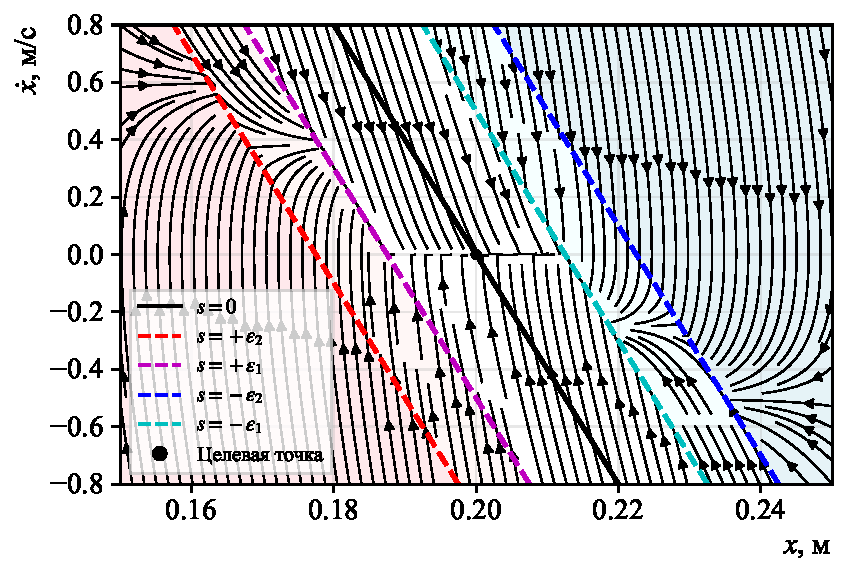
\includegraphics[]{part3/phase_portrait_5mode.pdf}
	\caption{Распределение векторного поля в фазовом пространстве для пятирежимного управления.
		Введение дополнительных режимов торможения создаёт более сложную структуру векторного поля с промежуточными зонами управления}
	\label{fig:vector_field_linear_5mode}
\end{figure}

Ключевое преимущество пятирежимного управления заключается в более плавном снижении скорости движения перед
включением режима удержания. Это позволяет уменьшить перерегулирование и снизить статическую ошибку без увеличения
частоты переключений. Также снижается вероятность возникновения «дребезга», поскольку система проходит
через промежуточные режимы торможения, что сглаживает переходы между режимами.

\textbf{Семирежимное управление.}
Дальнейшее развитие концепции многорежимного управления привело к разработке семирежимной схемы,
обеспечивающей ещё более тонкую градацию торможения перед достижением целевого положения.
Закон управления имеет вид:
\begin{equation}\label{eq:control_law_7_mode}
	\mathbf{u}(s) = \begin{cases}
		[1,0,0,1], & s > \varepsilon_3                     ; \\
		[1,0,0,0], & \varepsilon_2 < s \leq \varepsilon_3 ;  \\
		[0,0,0,1], & \varepsilon_1 < s \leq \varepsilon_2 ;  \\
		[0,0,0,0], & |s| \leq \varepsilon_1          ;       \\
		[0,1,0,0], & -\varepsilon_2 < s \leq -\varepsilon_1; \\
		[0,0,1,0], & -\varepsilon_3 < s \leq -\varepsilon_2; \\
		[0,1,1,0], & s \leq -\varepsilon_3,
	\end{cases}
\end{equation}
где $\varepsilon_1, \varepsilon_2, \varepsilon_3$ -- параметры, определяющие границы зон переключения режимов ($\varepsilon_1 < \varepsilon_2 < \varepsilon_3$).

Дополнительные режимы $[0,0,0,1]$ и $[0,1,0,0]$ обеспечивают слабое ускорение в положительном и
отрицательном направлениях, создавая ещё более плавный переход к режиму удержания. Векторное поле
в фазовом пространстве для семирежимного управления показано на рис.~\ref{fig:vector_field_linear_7mode}.

\begin{figure}[ht]
	\centering
	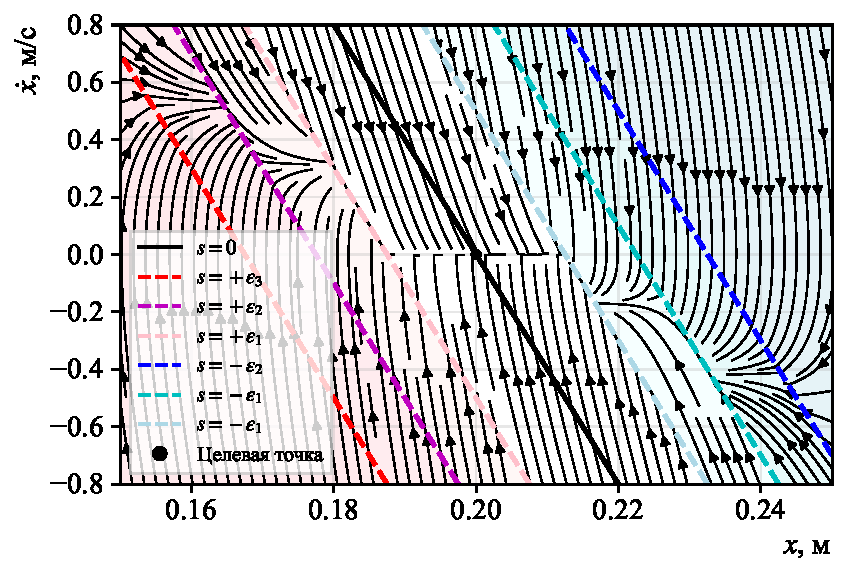
\includegraphics[]{part3/phase_portrait_7mode.pdf}
	\caption{Распределение векторного поля в фазовом пространстве для семирежимного управления.
		Градация режимов торможения создаёт более сложную, но эффективную структуру векторного поля
		с несколькими промежуточными зонами}
	\label{fig:vector_field_linear_7mode}
\end{figure}

Семирежимное управление обеспечивает наиболее плавное снижение скорости перед остановкой, что позволяет
достичь высокой точности позиционирования при минимальном количестве переключений распределителей.
Как показали результаты моделирования (подробнее в главе~\ref{ch:ch5}), данная схема обеспечивает наилучшее
сочетание точности позиционирования, быстродействия и ресурсных показателей по сравнению с трёх- и пятирежимным управлением.

\subsection*{Типы поверхностей скольжения}\label{subsec:ch3/sec3/sub3}

Эффективность управления в скользящих режимах существенно зависит от выбора поверхности скольжения.
В данном исследовании рассматриваются два основных типа поверхностей: интегральная и терминальная.

\textbf{Интегральная поверхность скольжения.}
Интегральная поверхность скольжения описывается уравнением \cite{sliding_surface_integral}:
\begin{equation}
	s_I = \dot{e} + \lambda_1 e + \lambda_2 \int_0^t e(\tau)d\tau,
\end{equation}
где $\lambda_1$ и $\lambda_2$ -- положительные коэффициенты.

Главное отличие интегральной поверхности от линейной заключается в наличии интегральной составляющей,
которая обеспечивает нулевую статическую ошибку в установившемся режиме. Это особенно важно для
позиционных систем, где требуется высокая точность позиционирования.

При движении вдоль интегральной поверхности динамика ошибки описывается дифференциальным уравнением второго порядка:
\begin{equation}
	\ddot{e} + \lambda_1 \dot{e} + \lambda_2 e = 0.
\end{equation}

Характер переходного процесса зависит от соотношения коэффициентов $\lambda_1$ и $\lambda_2$:
\begin{itemize}
	\item при $\lambda_1^2 > 4\lambda_2$ система демонстрирует апериодический характер движения;
	\item при $\lambda_1^2 < 4\lambda_2$ -- колебательный процесс;
	\item при $\lambda_1^2 = 4\lambda_2$ -- критический апериодический процесс (оптимальное соотношение).
\end{itemize}

\textbf{Терминальная поверхность скольжения.}
Терминальная поверхность скольжения представляется выражением \cite{sliding_surface_terminal}:
\begin{equation}
	s_T = \dot{e} + \beta |e|^{q/p} \text{sign}(e),
\end{equation}
где $p$ и $q$ -- нечетные числа, удовлетворяющие условию $1 < q/p < 2$; $\beta$ -- положительный коэффициент.

Главная особенность терминальной поверхности -- обеспечение конечного времени сходимости ошибки к нулю.
При движении вдоль терминальной поверхности динамика ошибки описывается нелинейным дифференциальным уравнением:
\begin{equation}
	\dot{e} = -\beta |e|^{q/p} \text{sign}(e).
\end{equation}

Время сходимости ошибки к нулю можно вычислить аналитически:
\begin{equation}
	T_f = \frac{p}{\beta(p-q)}|e(0)|^{1-q/p}.
\end{equation}

Ключевое преимущество терминальной поверхности -- ускорение сходимости при малых ошибках.
Поскольку $q/p > 1$, то при $e \to 0$ скорость сходимости ошибки увеличивается, что обеспечивает
более быстрое достижение целевого положения по сравнению с линейной или интегральной поверхностями.
Это особенно важно для прецизионных систем, где требуется высокая точность позиционирования.

На рис.~\ref{fig:smc_terminal} представлены результаты моделирования системы с терминальной
поверхностью скольжения при $p = 9$, $q = 11$ и $\beta = 5$. Как видно из графиков, система
быстро достигает целевого положения без перерегулирования, демонстрируя высокую точность позиционирования.

\begin{figure}[ht]
	\centering
	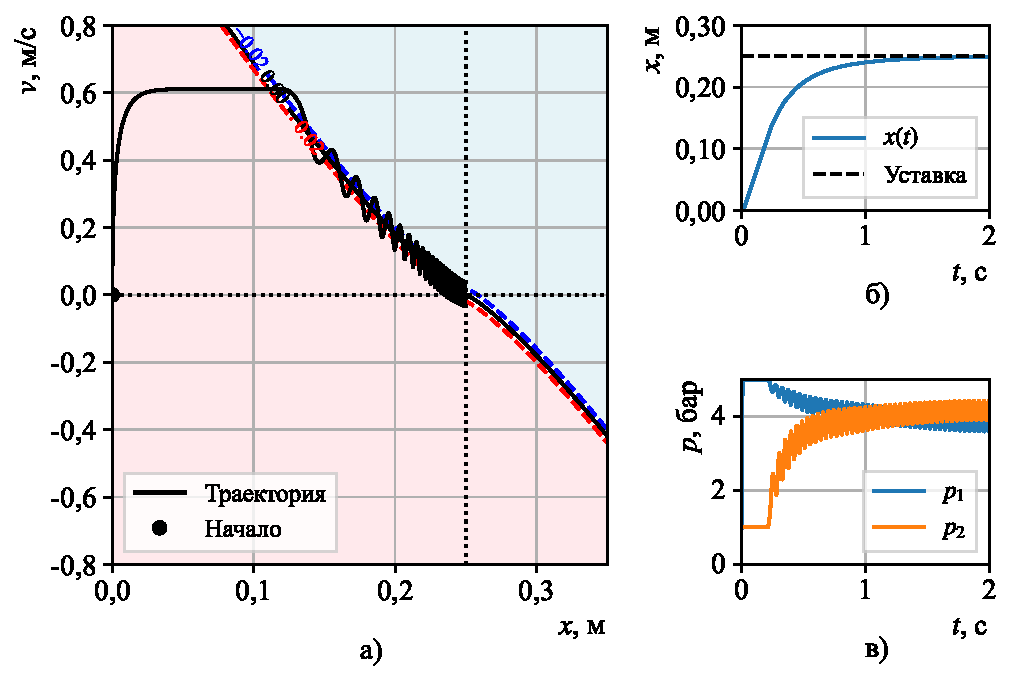
\includegraphics[]{part3/smc_teminal.pdf}
	\caption{Динамика системы с терминальной поверхностью скольжения
		при $p=9$, $q=11$ и $\beta=5$: а) фазовый портрет; б) переходной процесс; в) изменение давлений в полостях}
	\label{fig:smc_terminal}
\end{figure}


Анализ различных конфигураций многорежимного управления в скользящих режимах позволяет сделать следующие выводы:

\begin{enumerate}
	\item Трёхрежимное управление, хотя и обеспечивает достижение целевого положения, но имеет существенные
	      ограничения в точности позиционирования и стабильности процесса из-за компромисса между шириной $\varepsilon$-окрестности
	      поверхности скольжения и вероятностью возникновения «дребезга».

	\item Пятирежимное управление за счёт введения промежуточных режимов торможения позволяет существенно
	      улучшить характеристики процесса позиционирования, обеспечивая более плавное снижение
	      скорости и снижение статической ошибки без увеличения частоты переключений распределителей.

	\item Семирежимное управление обеспечивает наилучшие показатели качества позиционирования
	      среди рассмотренных конфигураций, создавая оптимальную градацию торможения перед достижением целевого положения.

	\item Интегральная поверхность скольжения обеспечивает нулевую статическую ошибку в
	      установившемся режиме и высокую робастность к постоянным возмущениям, что делает её предпочтительной для систем, работающих в условиях внешних нагрузок.

	\item Терминальная поверхность скольжения обеспечивает конечное время сходимости и
	      ускоренную сходимость при малых ошибках, что делает её предпочтительной для прецизионных систем с высокими требованиями к точности позиционирования.
\end{enumerate}

Выбор конкретной конфигурации (количество режимов и тип поверхности скольжения) должен осуществляться с учётом
требований к точности позиционирования, быстродействию и ресурсным показателям системы. Для этого в главе~\ref{ch:ch5} будет
представлена методика структурно-параметрического синтеза, позволяющая определить оптимальные параметры управления в зависимости от заданных критериев оптимизации.